%! Author = Philipp Emmenegger
%! Date = 14/07/2021

\section{Lambda Calculus}
\begin{itemize}
    \item Indroduced by Alonzo Church in 1930s
    \item Part of an investigation into the foundations of mathematics
    \item Expresses computation based on function abstraction
    \item Expresses application using variable binding and substitution
    \item Most compact and elegant programming language
    \item Basics for functional programming
    \item \textbf{Pure:} no pre-defined constants
    \begin{itemize}
        \item Only reserved words: '$\lambda$', '.', '(' and ')',
    \end{itemize}
    \item Proofs that function evaluation is enough for functional programming
\end{itemize}

\subsection{Sequents in LC}
Sequents in \textbf{LC} have the identical form as in\\
\textbf{PC} (Propositional Calculus) and \\ 
\textbf{FoPCe} (First-Order Predicate Calculus with Equality).\\
\begin{center}
    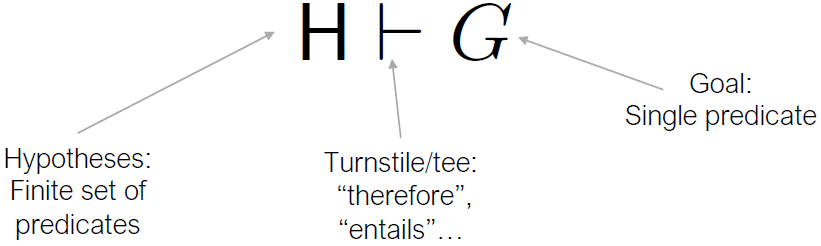
\includegraphics[width=0.8\linewidth]{img/sequents_lc.png}\\
    \textbf{\textit{Under the hypotheses H, prove the goal G}}
\end{center}

\subsection{Syntax in LC}
Formulae in LC can eiter be:
\begin{itemize}
    \item predicates (P)
    \item $\lambda$-Terms (M)
\end{itemize}
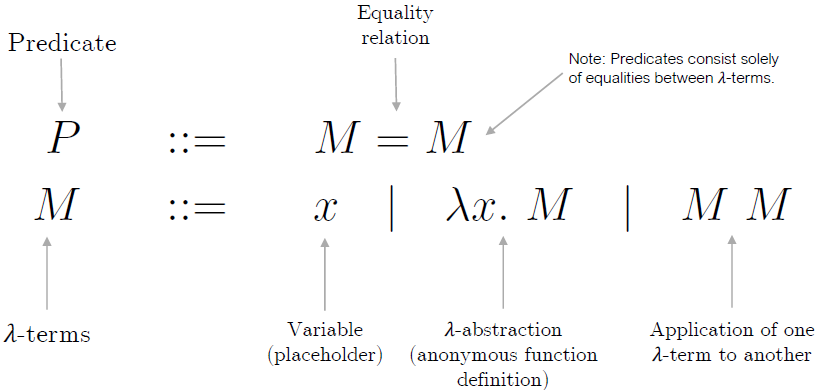
\includegraphics[width=\linewidth]{img/lc_syntax.png}

\subsubsection{Conventions}
\textbf{Application binds tighter than abstraction}\\
$\lambda x.M_1 M_2$ represents $\lambda x.(M_1M_2)$ and not $(\lambda x.M_1) M_2$\\ 
\textbf{Application is left associative}\\ 
$M_1 M_2 M_3$ represents $(M_1 M_2) M_3$ and not $M_1 (M_2 M_3)$

\subsubsection{Free and Bound Variables}
Bound variables are basically placeholders. 
Their names have no significance and can be renamed.\\
\begin{center}
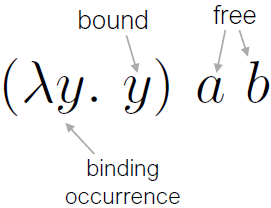
\includegraphics[width=0.2\linewidth]{img/lc_variables.png}
\end{center}
\textbf{$\alpha$-equivalence:}\\
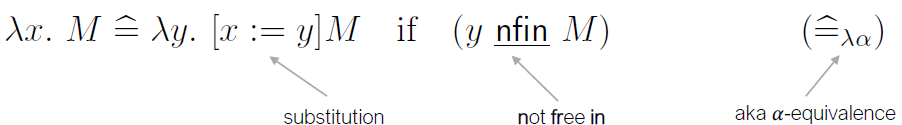
\includegraphics[width=\linewidth]{img/lc_alpha.png}

\subsubsection{Proof rules of LC}
Lambda Calculus contains only one proof rule schema of major significance: \textbf{$\beta$-reduction}\\ 
\begin{center}
    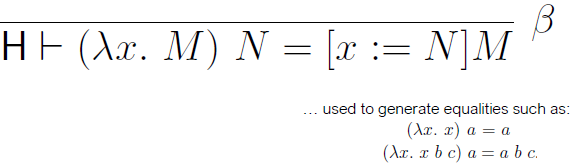
\includegraphics[width=0.8\linewidth]{img/lc_beta.png}
\end{center}
$\beta$-Reduction defines what function application means in the context of lambda calculus. 
It states that applying a lambda abstraction $(\lambda x.M)$ to another lambda term $(N)$ results in all occurences of the formal parameter $(x)$ within the body of the abstraction $(M)$ being replaced with the actual parameter $(N)$ supplied.\\\\ 
\begin{center}
    $\frac{(\lambda x. \; square \; x)\; 5}{=\; square \; 5}$\\
    \vspace{0.5cm}
    $\frac{(\lambda x. \; square \; x) \: (\lambda y. \; square \; y) \; 5}{= \; (square \; (\lambda y. \; square \; y)) \; 5}$
\end{center}

\subsection{Computation with LC}
Computation in the lambda calculus is done by repeatedly applying the rule schema $\beta$ to achieve $\beta$-reduction.\\ 
\begin{center}
    \textbf{Evaluation in LC = Reduction}
\end{center}

\subsubsection{Normal Form}
A $\lambda$-term is said to be in \textbf{normal form} if no further reductions can be applied to it.
It is possible for a $\lambda$-term to offer several opportunities for reduction simultaneously:
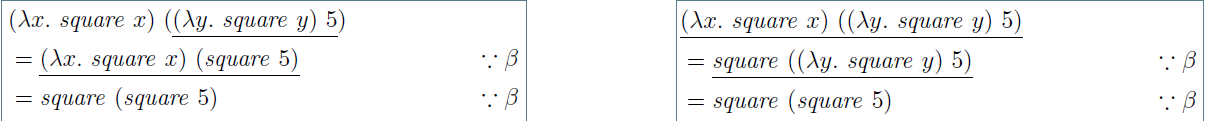
\includegraphics[width=\linewidth]{img/lc_reduction.png}
\textbf{Confluence:} Every $\lambda$-term has at most one normal form

\subsubsection{Function Application Syntax}
Functions are \textbf{first-class citizens}. Functions and their arguments belong to the same syntactic category.
\begin{itemize}
    \item Prefix notation is used instead of infix notation
    \item Parameters do not need to be enclosed in parantheses
\end{itemize}

\subsubsection{Currying}
\textbf{Motivation:} LC only allows unary (1 argument) function application.\\ 
\textbf{Currying:} A function with several arguments can be thought of as a series of higher order functions, each with being unary.
\begin{itemize}
    \item Not just a smart syntactic trick
    \item Makes functional definitions more concise, modular and reusable
\end{itemize}

\subsubsection{Definitions}
\begin{itemize}
    \item Not strictly necessary 
    \item Sometimes convenient
    \item Adding definitions as equalities within the hypotheses of LC sequents
\end{itemize}
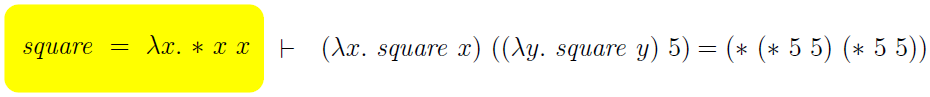
\includegraphics[width=\linewidth]{img/lc_definitions.png}

\subsubsection{Delta-Reduction}
\textbf{$\delta$-Reduction:} substitution of a defined symbol with its definition\\
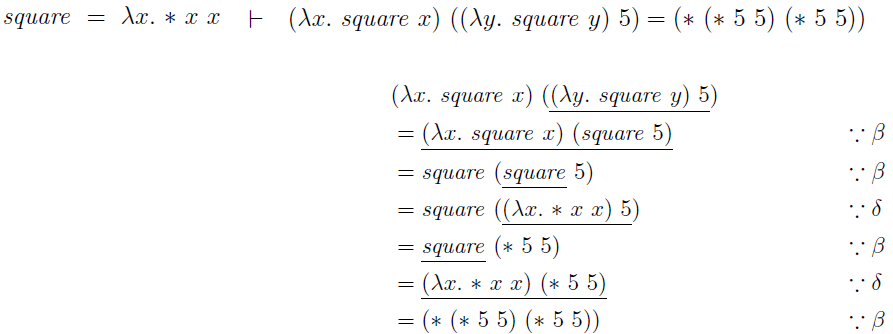
\includegraphics[width=\linewidth]{img/lc_delta.png}

\subsection{Evaluation Strategies}
\textbf{redex:} reducible expression (any $\beta \delta$-reducible sub-term)\\ 
\textbf{evaluation strategy:} order in which redexes are reduced
\begin{itemize}
    \item $\lambda$-terms may have more than one redex at any stage of the evaluation
    \item LC does not place any constraints on the order in which redexes are reduced
    \item The order plays an important role in the \textbf{length of derivations} and their \textbf{termination}
\end{itemize}

\subsubsection{Leftmost Innermost (aka. applicative order / innermost first)}
\begin{enumerate}
    \item The innermost redex is reduced First
    \item In case there is more than one innermost redex, the leftmost innermost redex is reduced First
\end{enumerate}
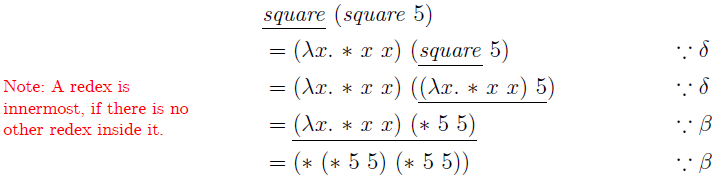
\includegraphics[width=0.9\linewidth]{img/lc_innermost.png}
\begin{itemize}
    \item A functions arguments are substituted into the body of a function after they are reduced
    \item A functions arguments are reduced exactly once
    \item Parameter passing: \textbf{Call by value}
\end{itemize}

\subsubsection{Leftmost Outermost (aka. normal order / outermost first)}
\begin{enumerate}
    \item The outermost redex is reduced First
    \item In case there is more than one outermost redex, the leftmost-outermost redex is reduced First
\end{enumerate}
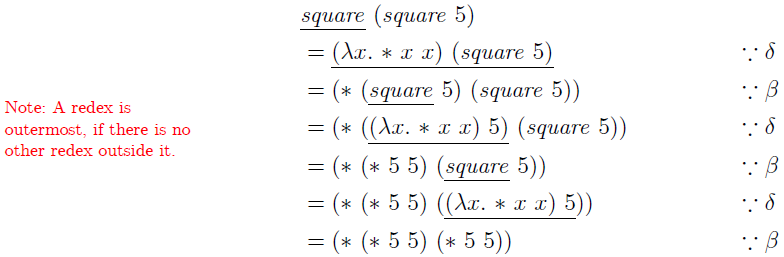
\includegraphics[width=0.9\linewidth]{img/lc_outermost.png}
\begin{itemize}
    \item A functions arguments are substituted into the body of a function before they are reduced
    \item A functions arguments are reduced as often as they are needed
    \item \textbf{If a normal form exists, leftmost outermost will find it}
    \item Parameter passing: \textbf{Call by name}
\end{itemize}

\subsubsection{Lazy Evaluation}
Implementation technique to make call by name more efficient.
Uses memorizing (caching) to avoid computing the same expression more than once.
\textbf{Default for Haskell}

\subsection{Encoding Data and Operations}
The pure lambda calculus \textbf{does not have any primitive data types} such as Booleans, numbers, tuples, etc.\\ 
\subsubsection{Boolean Algebra}
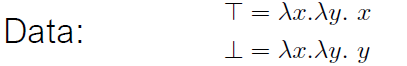
\includegraphics[width=0.5\linewidth]{img/lc_data.png}
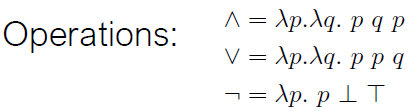
\includegraphics[width=0.5\linewidth]{img/lc_operations.png}
\subsubsection{Arithmetic}
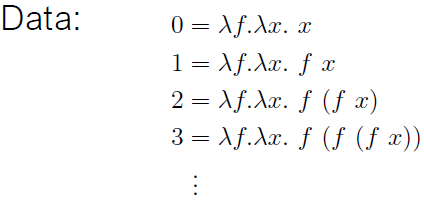
\includegraphics[width=0.35\linewidth]{img/lc_data2.png}
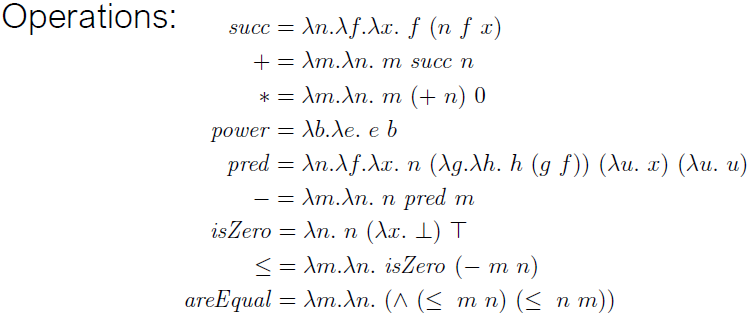
\includegraphics[width=0.65\linewidth]{img/lc_operations2.png}
\subsubsection{Pairs}
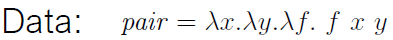
\includegraphics[width=0.5\linewidth]{img/lc_data3.png}
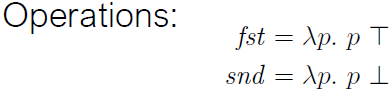
\includegraphics[width=0.5\linewidth]{img/lc_operations3.png}